\chapter[Resultados Parcias ]{Resultados Parciais}

\section{Resultados obtidos em MATLAB}
Em 2010 fabien lotte publicou um trabalho, demosntrando a classificação de sinais de EEG com LDA(paperlotte),usando o estrator de características common spatial pattenrs (CSP) e outras
variações deste algoritmo. A base de dados usada foi a base do BCI competition III, com os datasets BCI\_III\_DSIVa, BCI\_III\_DSIIIa e BCI\_IV\_DSIIa. 

As implementações foram codificadas em Matlab, e o autor chegou aos seguintes resultados mostrados na tabela .

%\begin{figure}[h]
%	\centering
%	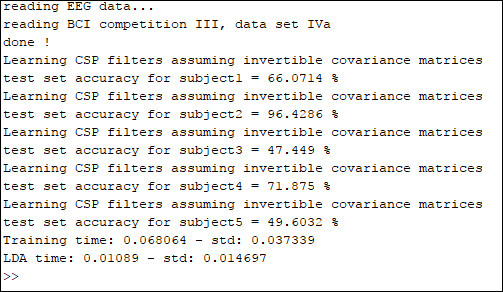
\includegraphics[keepaspectratio=true,scale=1.0]{figuras/resultados_csp_lda.png}
%	\caption{Resultados obtidos  com CSP-LDA}
%	\label{resultadoLotte}
%\end{figure}
 
Reproduzir os resultados do autor, é de suma importância para este trabalho, tanto para comparação quanto para o entendimento do algoritmo. Ao executar o os códigos desenvolvidos por Lotte, em um laptop DELL, equipado com processador Intel Core I5-4210U CPU 2.4 GHz, 8 GB RAM, ultilizando os mesmos datasets, obteve-se os resultados contidos na tabela

